\fcolorbox{red}{yellow}{esto no va aca}
\subsubsection{Configuración de comunicación CANopen}

\begin{tcolorbox}[colback=blue!5!white,colframe=blue!75!black,title=CANopen]
	CANopen es un protocolo con aplicación industrial de bajo nivel para aplicaciones de automatización. Conecta dispositivos entre sí mediante mensajes entre pares. Basado en el estándar de comunicaciones físicas CAN. Se utiliza en redes de comunicación tipo esclavo, multimaestro. \fcolorbox{red}{yellow}{no me cierra esta definicion, buscar otra}
\end{tcolorbox}


\paragraph{Registros a utilizar}
\fcolorbox{red}{yellow}{ir a ANEXO y poner la lista completa de direcciones}

\subsubsection{Comunicación}
\fcolorbox{red}{yellow}{poner el diagrama}//
\fcolorbox{red}{yellow}{falta leer esto y acomodar}
El   variador   también   se   puede   controlar   en   modo   remoto.   Es   adecuado   paraaplicaciones en   los   que   los   cambios   de   variables   del   variadorse   realizan frecuentemente  durante  el proceso.  Dichos  cambios  pueden  realizarse  por  parte  del propio  operario  (mediante  potenciómetros,  interruptores,  selectores  rotativos  o  BCD, etc.).  Sin  embargo,  la  situación  más  común  es  que  los  parámetros  del  variador  los establezca  el  equipo  de  control  y  supervisión  del  proceso,  al  que  está  conectado  el variadorde  frecuencia: reguladores  de  tensión  y/o  corriente,  finales  de  carrera, pantallas de operador, etc., o incluso un ordenador personal y/o PLC. Para  el  casode  estos  controles  remotos,  la  comunicación  se  puede  realizarde  dos modos:\\Mediante un  número  determinado  de  conductores,  que  depende  de  los elementos que se tengan conectados al variador de frecuencia, por el que se transmiten señales digitales (finalesde carrera, interruptores, salidas digitales de un PLC), o analógicas (potenciómetro, salida analógica de un PLC):\\Mediante un bus de comunicaciones industriales (de 2 o 4 hilos), sobre el que se transmiten   mensajes   de   ajuste   de   parámetros   siguiendo   un   protocolo preestablecido (Modbus, CanBus, ProfiBus, EtherCat, etc.).Con 2  conductores la  comunicación  se  hace  más  lenta(modo  semidúplex),  pero  lógicamente representa un menor coste.

\begin{figure}[htb]
	\centering
	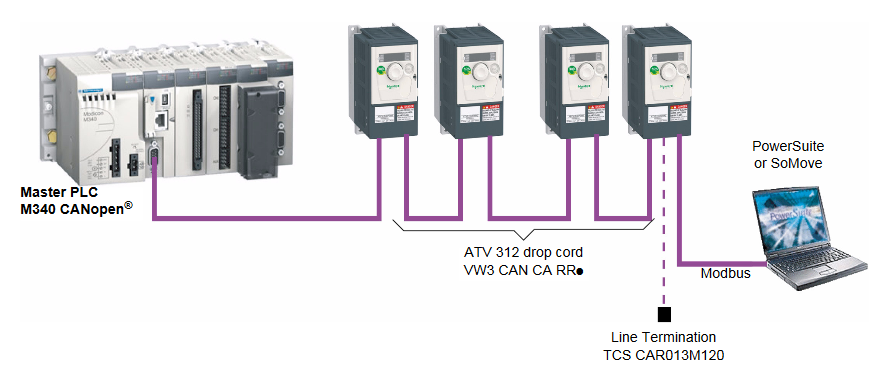
\includegraphics[scale=0.7]{comu.png}
	%\caption{Placa BME280}
	%\label{fig:BME280}
\end{figure}


\paragraph{Configuración CANopen}

\fcolorbox{red}{yellow}{imagenes. y paso a paso}\\
\\

\paragraph{Configuración Modbus}
\begin{tcolorbox}[colback=blue!5!white,colframe=blue!75!black,title=ModBus]
	Modbus es un protocolo de comunicaciones utilizado para transmitir información a través de redes en serie entre dispositivos electrónicos, basado en la arquitectura maestro/esclavo o cliente/servidor, diseñado en 1979 por Modicon para su gama de PLC. Convertido en un protocolo de comunicaciones estándar en la industria. Además, esta red de comunicación industrial usa los protocolos RS232/RS485/RS422.
	%http://microelecblog.blogspot.com/2013/12/configuracion-atv312-para-red-modbus.html
\end{tcolorbox}
\fcolorbox{red}{yellow}{imagenes. y paso a paso}

%EL ERROR QUE TENIA CRISTIAN con ifix SE ARREGLO CON ESTO
%\url{http://www.cimexcorp.com/hasp_fix.htm}